\subsection{Standard mechanical components}

%---------------------- SEALS AND WATERPROOFING ----------------------%

\subsubsection{Seals and Waterproofing}
\sssubsection{Static Seals for Enclosures} \mbox{}\\

To provide a weatherproof chassis or enclosure, many components and methods can be used. The first is the use of O-rings in compression to seal elements such as fasteners or buttons. A sealing fastener with O-ring is shown in Figure \ref{fig:seal_fastener}. This is an adequate method to keep water and contaminants out of the enclosure \cite{fastenright_sealing_nodate}.

\begin{figure}[H]
    \centering
    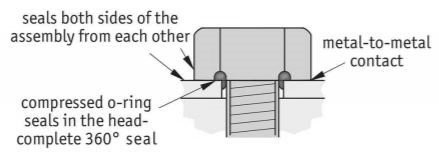
\includegraphics[width=0.7\textwidth]{Sections/LiteratureReview/img/seals/seal_fastener.JPG}
    \caption{Possible gasket configurations and mounting \cite{automotion_components_integral_nodate}}
    \label{fig:seal_fastener}
\end{figure}

O-rings often fall in the broader category of gaskets, which are compressible materials that can be added between parts. The compression is often achieved by a mechanical method such as bolting the parts together \cite{ali_m._sadegh_marks_2018}. Gaskets are available in many shapes, sizes and materials, and can be custom made \cite{protocase_custom_nodate}. An example of available materials for custom made gaskets (from Protocase manufacturer) is shown in Appendix \ref{app:gaskets}. Some gasket mounting configurations are shown in Figure \ref{fig:gasket_final}.

\begin{figure}[H]
    \centering
    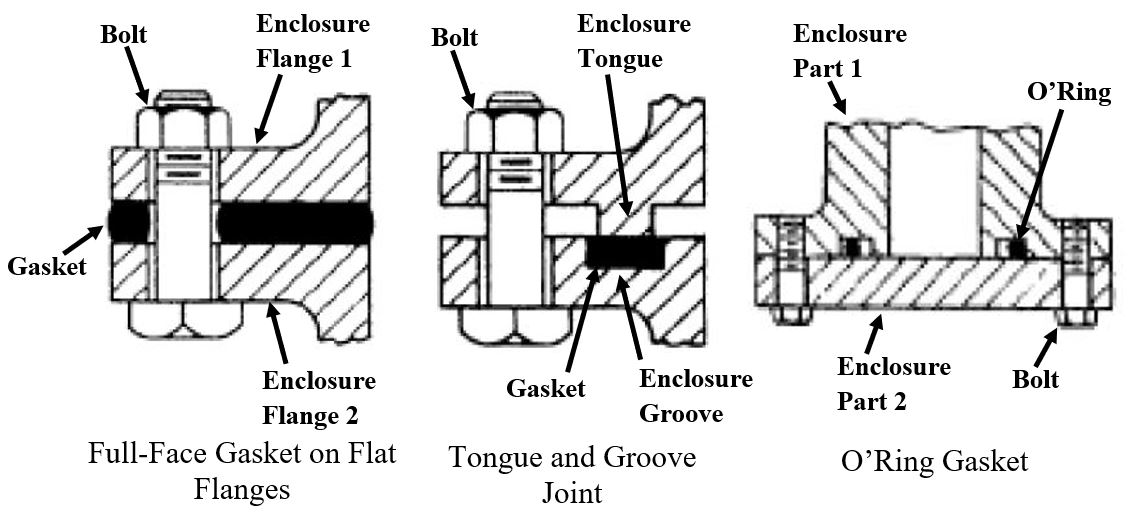
\includegraphics[width=0.7\textwidth]{Sections/LiteratureReview/img/seals/gasket_final.JPG}
    \caption{Possible gasket configurations and mounting \cite{ali_m._sadegh_marks_2018}}
    \label{fig:gasket_final}
\end{figure}

An additional option is liquid sealants. These are used in a similar way as gaskets, but are applied in the liquid form onto the parts, and harden after the assembly has been completed. This allows them to take the shape of the gap. Generally the solidification is done through a chemical reaction, which can be anaerobic \cite{henkel_improving_nodate}. Their advantage is that they can be easily formed in the required shape, and can be re-applied if broken for maintenance purposes. Many materials, such as silicone, polyurethane and various polymer sealants are available. Each provide various properties, which can include resistance to marine environments and UV-radiation \cite{3m_sealants_nodate}. Figure shows the application of the liquid sealant, while taking care to circle around any fastener holes \cite{henkel_improving_nodate}.

\begin{figure}[H]
    \centering
    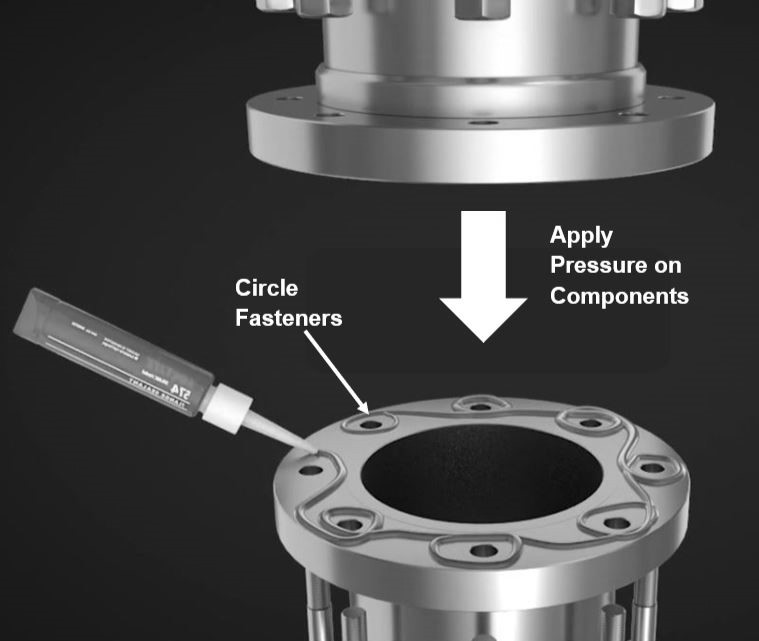
\includegraphics[width=0.7\textwidth]{Sections/LiteratureReview/img/seals/seal_liquid.JPG}
    \caption{How to seal components using liquid sealant \cite{henkel_improving_nodate}}
    \label{fig:seal_liquid}
\end{figure}



%---------------------- DYNAMIC SEALS FOR EXTERIOR COMPONENTS ----------------------%

\sssubsection{Dynamic Seals for Exterior Components} \mbox{}\\

The waterfront robot could have sensible elements located on its exterior, for example on the legs. These must be protected from the elements using some form of barrier. "Interior" style rotary shaft seals and seals for reciprocating motion elements (such as pistons) are likely not to be used in this application as they are more useful for continuously rotating joints or are considered integral parts of off-the-shelf components. Some options and explanations are shown in Appendix \ref{app:dynamicseals}. 

The focus is to shield expanding and flexible components such as linkages and moving joints. Molded bellows can be used to cover the assembly. They are available in many shapes and materials (including waterproof and custom options) and are often corrugated to provide angular and linear flexibility (see Figure \ref{fig:bellow_types}). They can be mounted using hose clamps or by using a backing plate bolted to the assembly, as shown in Figure \ref{fig:bellow_mount} \cite{hydraulics_&_pneumatics_protect_2012}.

\begin{figure}[H]
    \centering
    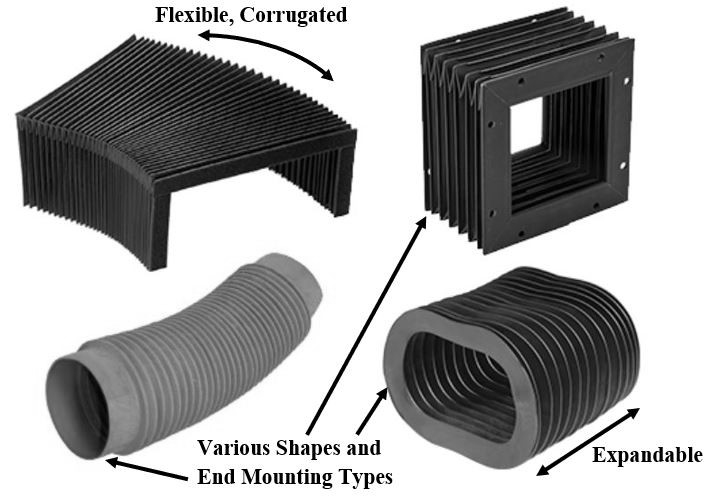
\includegraphics[width=0.7\textwidth]{Sections/LiteratureReview/img/seals/bellow_types.JPG}
    \caption{Various bellow cover types and shapes \cite{dynatec_bellows_nodate}}
    \label{fig:bellow_types}
\end{figure}

\begin{figure}[H]
    \centering
    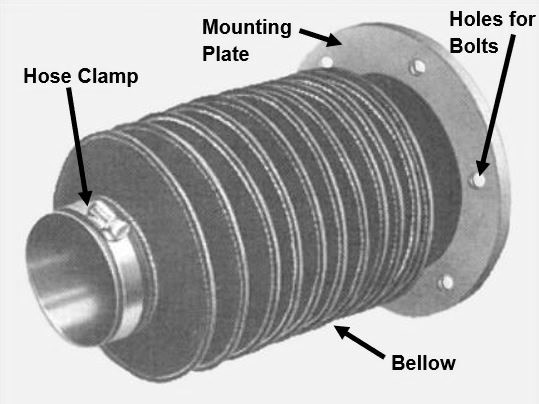
\includegraphics[width=0.5\textwidth]{Sections/LiteratureReview/img/seals/bellow_mount.JPG}
    \caption{Mounting options for bellow cover \cite{hydraulics_&_pneumatics_protect_2012}}
    \label{fig:bellow_mount}
\end{figure}

%------------------------ Bearings ------------------------%

\subsubsection{Bearings}

Stanford Doggo's knee joints uses two TRB rubber seal ball bearings and a steel shoulder bolt for rotation; this configuration works for them since the legs do not have abduction/adduction movement, resulting in zero axial stress on the bearings/bolt \cite{kau_nate711/stanforddoggoproject_2019}.

\begin{figure}[H]
    \centering
    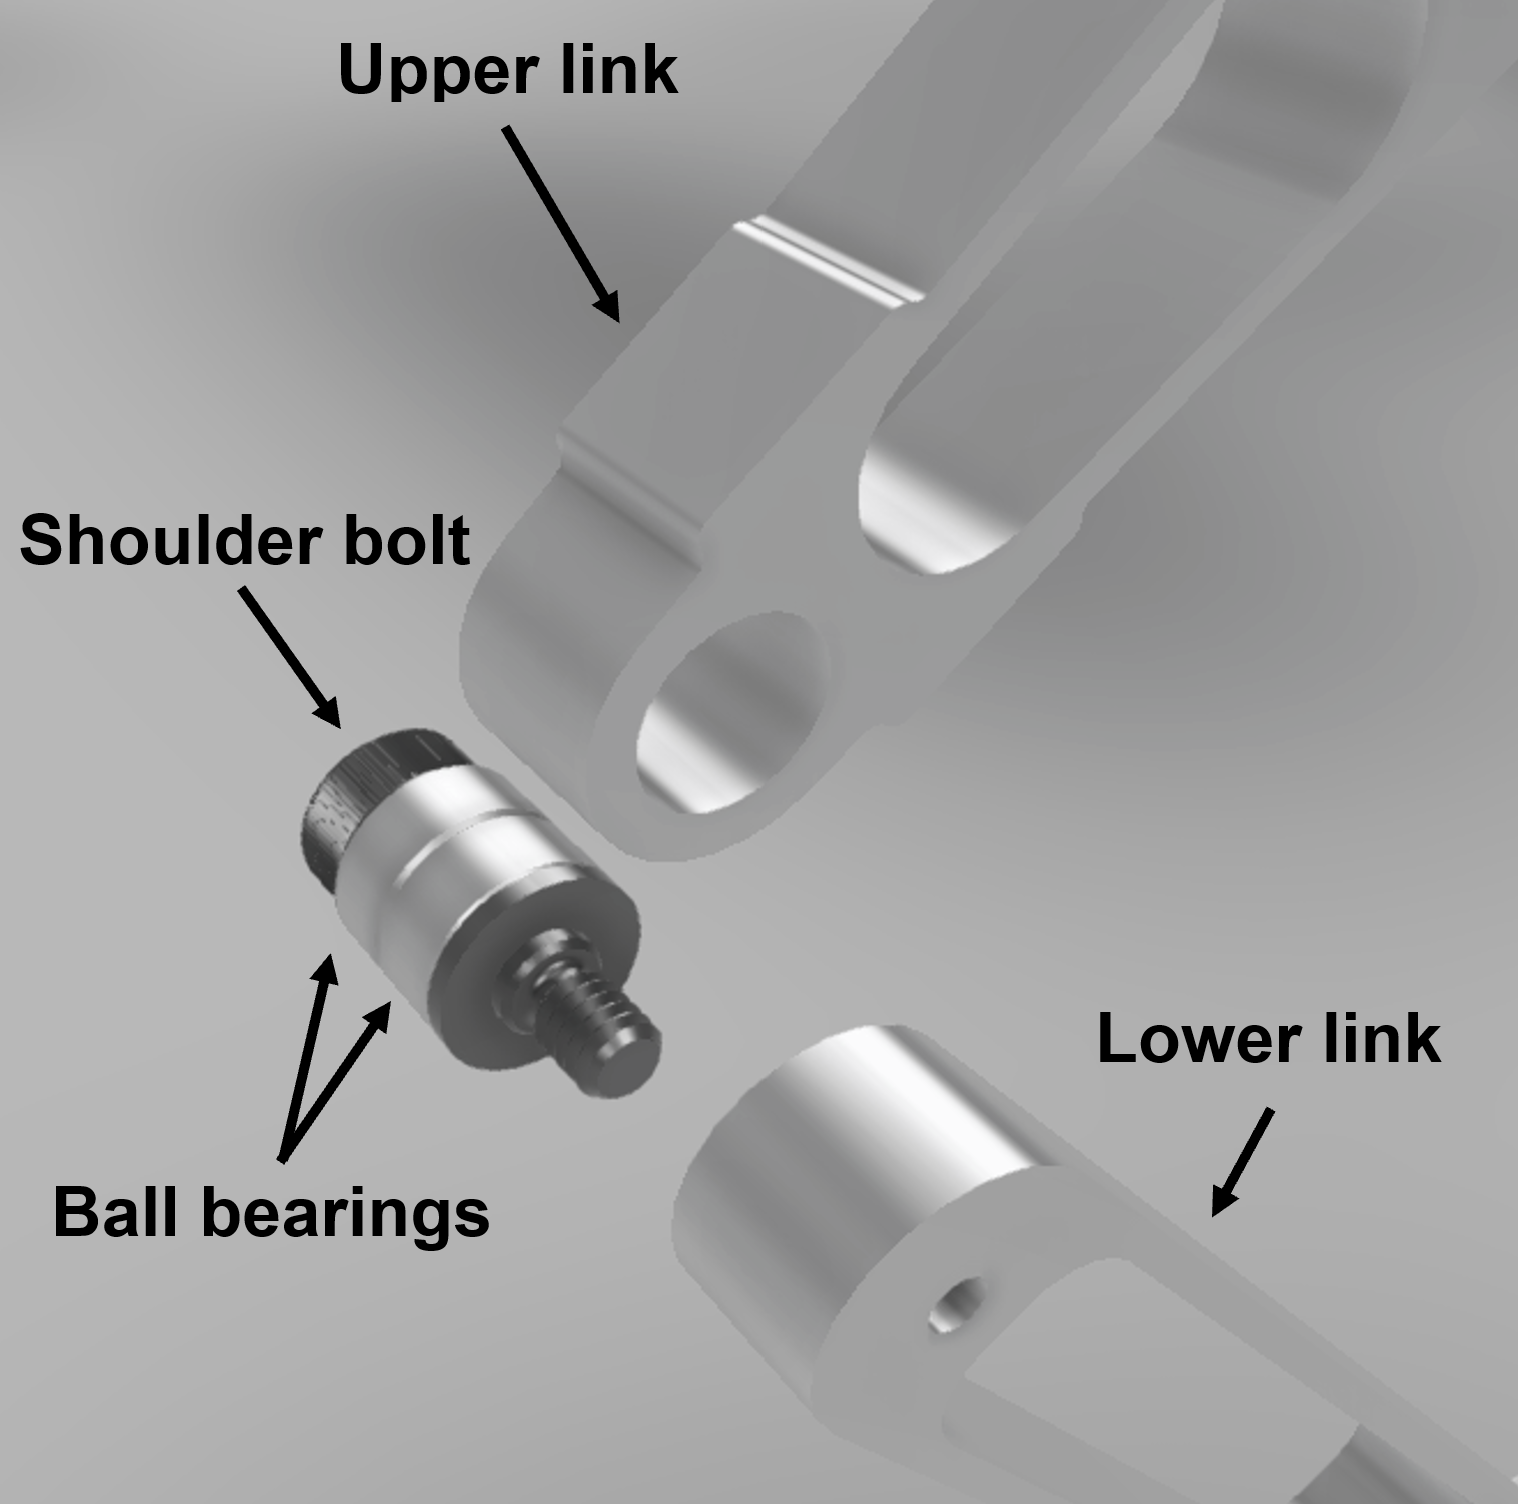
\includegraphics[width=0.49\textwidth]{Sections/LiteratureReview/img/doggo/subsys_doggo_knee.png}
    \caption{Stanford Doggo knee \cite{kau_nate711/stanforddoggoproject_2019}}
    \label{fig:doggo_knee}
\end{figure}

On a general point of view, bearings are used in nearly every situation where a rotary motion is produced and transferred onto a system. Bearings need to be mounted in such a way that the shaft or the bearings do not slide during the operation of the system. There are many different ways to mount and position them based on the specific design. First, a bearing can either be mounted onto the shaft or inside the housing \cite{hch_bearing_mounting_2013}. Figure \ref{fig:bearing_inner} presents a common method of mounting a bearing on the shaft that consists of holding the bearing against the shaft shoulder and then securing it with a component such as a lock ring, a retaining ring, or a spacer.

\begin{figure}[H]
    \centering
    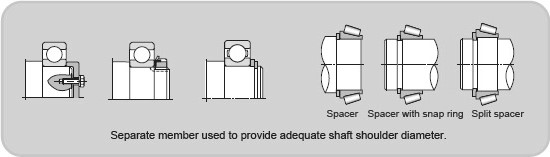
\includegraphics[width=0.9\textwidth]{Sections/LiteratureReview/img/Bearings/bearings_inner_set.jpg}
    \caption{Bearing inner ring mounting options \cite{hch_bearing_mounting_2013}}
    \label{fig:bearing_inner}
\end{figure}

The other option is to mount the outer ring of the bearing inside the housing using an end cap, an inner retaining ring, or a spacer as illustrated on Figure \ref{fig:bearing_outer}.

\begin{figure}[H]
    \centering
    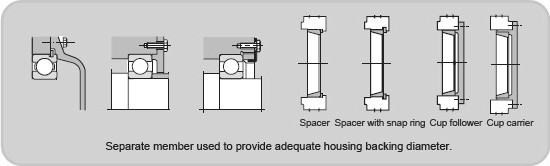
\includegraphics[width=0.9\textwidth]{Sections/LiteratureReview/img/Bearings/Bearings_outer_set.jpg}
    \caption{Bearing outer ring mounting options \cite{hch_bearing_mounting_2013}}
    \label{fig:bearing_outer}
\end{figure}

Combining both mounting options may be necessary based on the direction and magnitude of the axial forces. A common bearing mounting arrangement known as "fixed-floating" presented on Figure \ref{fig:bearing_fix-float} can be used to axially locate the shaft \cite{budynas_shigleys_2015}. This arrangement offers multiple options for the mounting devices of both the inner and outer races of the bearing. In this case, the left bearing is the only one that can take an axial load. Another bearing mounting arrangement known as "fixed-fixed", shown on Figure \ref{fig:bearing_fix-fix}, eliminates the use of mounting devices on the shaft which may create unwanted stress concentration points \cite{budynas_shigleys_2015}. This arrangement allows a single bearing to take the axial load from one direction. However, if the distance between the bearings is significant and the shaft elongates due to a rise in temperature, the bearings may fail due to the axial load in both directions created by the heat expansion of the shaft \cite{budynas_shigleys_2015}. This is why the fixed-floating arrangement from Figure \ref{fig:bearing_fix-float} is preferred in cases where high temperatures of operation are inevitable.

\begin{figure}[H]
    \centering
    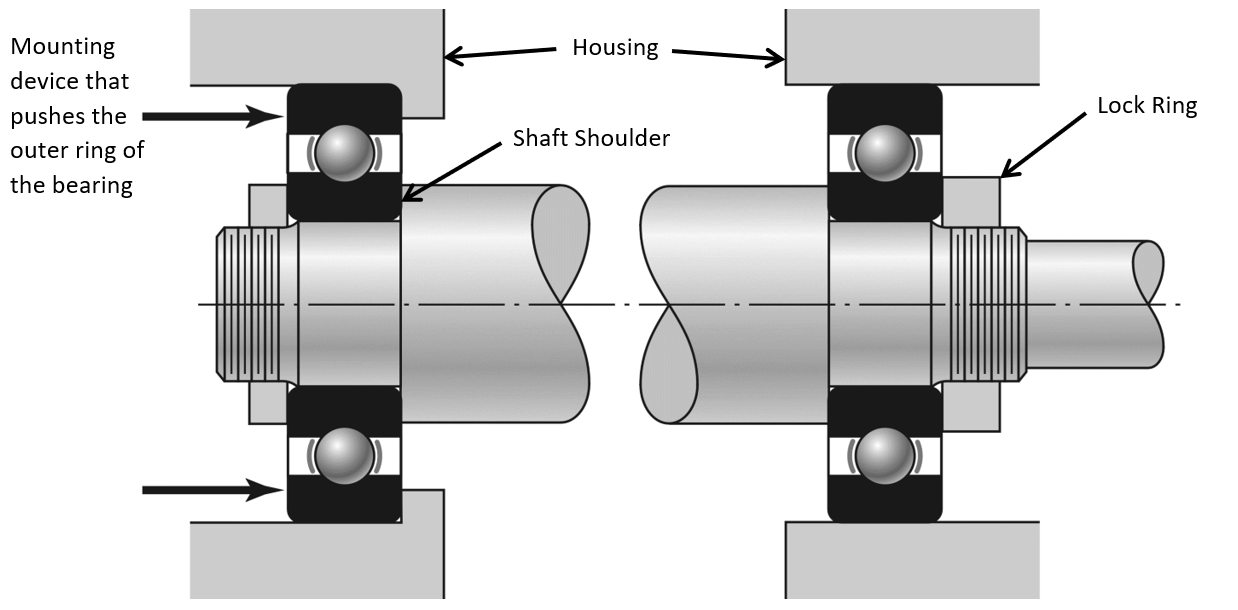
\includegraphics[width=0.85\textwidth]{Sections/LiteratureReview/img/Bearings/bearings_fix_float.png}
    \caption{Bearing fixed-floating mounting arrangement \cite{budynas_shigleys_2015}}
    \label{fig:bearing_fix-float}
\end{figure}

\begin{figure}[H]
    \centering
    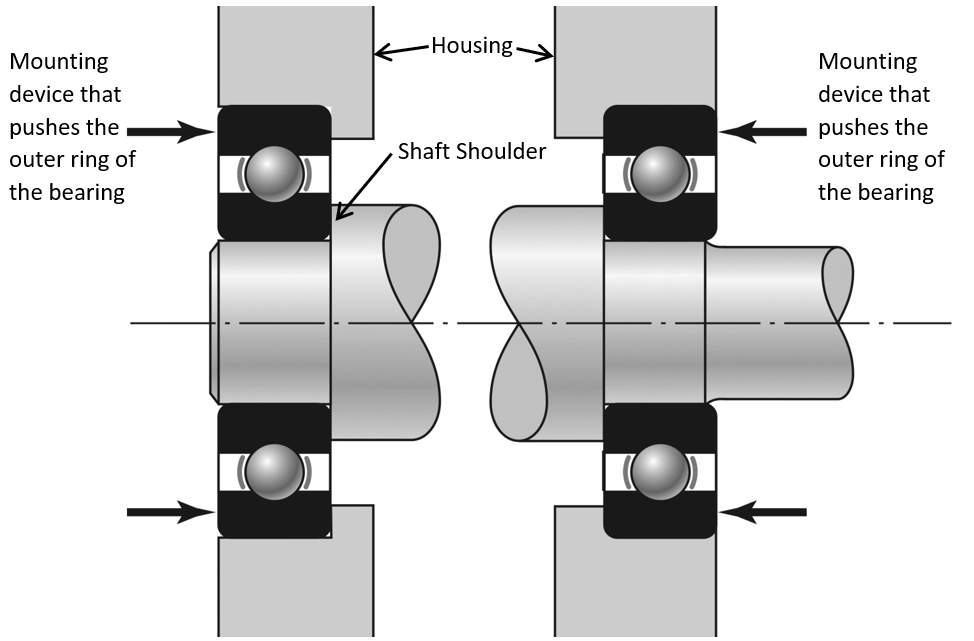
\includegraphics[width=0.75\textwidth]{Sections/LiteratureReview/img/Bearings/bearings_fix_fix.png}
    \caption{Bearing fixed-fixed mounting arrangement \cite{budynas_shigleys_2015}}
    \label{fig:bearing_fix-fix}
\end{figure}

If axial loads are significant, angular contact ball bearings or tapered roller bearings can be used instead of radial contact ball and roller bearings. When mounting such types of bearings, the direction of the axial load and the preloading method must be taken into considerations \cite{budynas_shigleys_2015}. Multiple options of mounting angular contact bearings are presented in Figure \ref{fig:bearing_arrang} in Appendix A.

%---------------------- ELECTRONICS ----------------------%

\subsubsection{Electronics}

All electronics shown in this section, with the exception of the MaxBotix MB7052 compact-housing, mount using basic metric screws and standoffs, as shown in Figure \ref{fig:nvidia_jetson}.

\sssubsection{Sensors} \mbox{}\\

The mandated robot must be self-sufficient; it must navigate the environment, avoid obstacles and identify trash without a human controlling it.
To do so, a set of sensors must be employed.
Common sensors used for robot navigation and balancing include GPS and IMUs, while sensors for obstacle avoidance include ultrasonic and laser proximity sensors \cite{corrigan_obstacle_2019}.

In the former category, GPS units sit on the robot and use satellites to identify the position of the robot.
Garmin offers a series of GPS units that are small and compact; the GPS 15x unit is 23.88 X 42.93 X 7.84 mm, weighs 7.37 g, mounts with 2 M2 screws, and consumes max 0.2625 W \cite{garmin_gps_2011}.
IMUs, or inertial measurement units, use gyroscopes and accelerometers to measure acceleration and rotation \cite{unmannedsystemstechnology_selecting_2018}.
This allows the robot to identify its orientation (such as determining whether it is on an incline, at risk of flipping over, etc.).
Inertial Sense offers compact all-in-one GPS/IMUs \cite{inertial_sense_imu_nodate}.
Their rugged $\mu$IMU costs \$800, is 16.5 X 12.6 X 4.6 mm, weighs 1.3 g and consumes 0.625 W. Figure \ref{fig:elec_IMUGPS} shows this GPS/IMU model, its relative size and mounting capabilities.
Individual IMUs can be purchased, such as the commonly used and inexpensive MPU-9250 \cite{sparkfun_sparkfun_nodate}.
It costs \$14.95, is 3 X 3 X 1 mm and consumes little to no power, as it feeds of that of an Arduino or equivalent board (and thus its power consumption is considered part of the microcontroller/computers).

\begin{figure}[H]
    \centering
    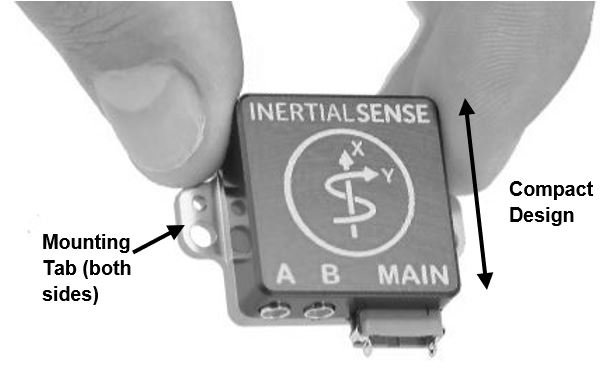
\includegraphics[width=0.5\textwidth]{Sections/LiteratureReview/img/electronics/elec_IMUGPS.JPG}
    \caption{Combination IMU/GPS by Inertial Sense \cite{inertial_sense_imu_nodate} }
    \label{fig:elec_IMUGPS}
\end{figure}

Laser or LiDAR sensors offer a greater range than ultrasonic sensors, but their performance degrades severely if the lens is wet, whereas ultrasonic sensors can operate underwater with appropriate software tweaks \cite{corrigan_obstacle_2019} \cite{garmin_lidar-lite_nodate}.
MaxBotix offers a suite of ultrasonic sensors suitable for waterfront environments.
Their MB7052 sensors are IP68 rated and have excellent corrosion resistance, as well as ranges between a few centimeters and 8 meters \cite{maxbotix_mb7052_nodate}.
The ultra-compact package type costs \$202.87, measures 30.48 X 35.56 X 25.27 mm, weighs 15.1 g and mounts with 4 M3 screws.
The compact housing package type also costs \$202.87, measures 34.7 X 34.7 X 38 mm, weighs 32 g and screws into a housing using a 3/4"-14 NPS. The package types and mounting capabilities are shown in Figure \ref{fig:elec_sonic} .
Garmin offers LiDAR (Light Detection and Ranging) sensors.
Their v3HP model is IPx7 compliant and offers up to 60m range \cite{garmin_lidar-lite_nodate}.
It costs \$150, measures 48 X 40 X 20 mm, weighs 22 g, mounts using 4 screws and consumes 0.425 W.

\begin{figure}[H]
    \centering
    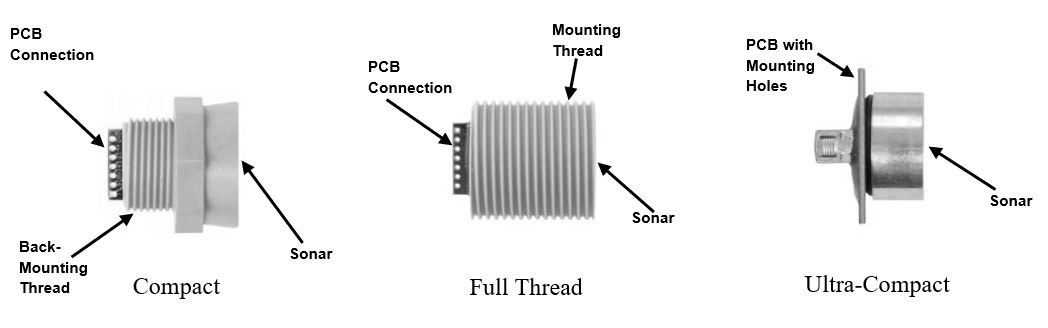
\includegraphics[width=0.9\textwidth]{Sections/LiteratureReview/img/electronics/elec_sonic.JPG}
    \caption{MaxBotix Ultrasonic Sensors Various Package Types \cite{maxbotix_mb7052_nodate} }
    \label{fig:elec_sonic}
\end{figure}

\sssubsection{Computing}\mbox{}\\

Robots rely on microcontrollers and full computers to compute path planning, image recognition, computer vision, and SLAM, amongst a host of other tasks.
Choosing the correct computer for a given application is important and can greatly impact the effectiveness of the robot.
There are a few popular computers on the market for robotics applications.

Arduino is a microcontroller designed for makers \cite{arduino_arduino_nodate}.
Built for simple tasks and instructions, it features a 16 Mhz processor and 0.232 W power draw at 5 V and 46 mA \cite{gadget_makers_blog_arduino_2013}.
It costs \$22, measures 68.6 X 53.4 mm, weighs 25 g and is mounted with 4 M3 screws \cite{elprocus_arduino_2019}. It's schematics are similar to those shown in Figure \ref{fig:nvidia_jetson}.

Raspberry Pi is a single-board computer, whose 4th generation was released this year \cite{raspberry_pi_raspberry_nodate}.
They have been used in a plethora of robots, including the Hexapod v2 \cite{smallp_tsai_hexapod_2018}.
Running at 5 V and requiring a 3 A power supply, the Raspberry Pi 4 pulls 1 A, or 5 W \cite{raspi.tv_how_2019}.
It costs \$55, measures 88 X 58 X 19.5 mm, weighs 46 g and is mounted with 4 M2.5 screws \cite{piltch_raspberry_2019} \cite{raspberry_pi_raspberry_nodate}.
Although offering more than double the performance of the previous generation of Raspberry Pi, its lack of a dedicated GPU unit reduces its usefulness for computer vision applications \cite{pulli_realtime_2012}.

The NVIDIA Jetson TX2, shown in Figure \ref{fig:nvidia_jetson}, is a machine learning oriented single-board computer with dedicated GPU for accelerated machine learning and computer vision tasks \cite{nvidia_jetson_2017}.
It offers nearly double the performance of the Raspberry Pi 4 for general compute tasks and likely 6 or more times the performance for computer vision applications, while consuming 7.5 W of power at 9-12 V \cite{pulli_realtime_2012} \cite{larabel_initial_nodate} \cite{larabel_benchmarks_2017} \cite{nvidia_jetson_2017-1}.
It costs \$479, measures 87 X 59 X 10 mm, weighs 88 g and is mounting with 4 M3 screws \cite{nvidia_jetson_2018}.

\begin{figure}[H]
    \centering
    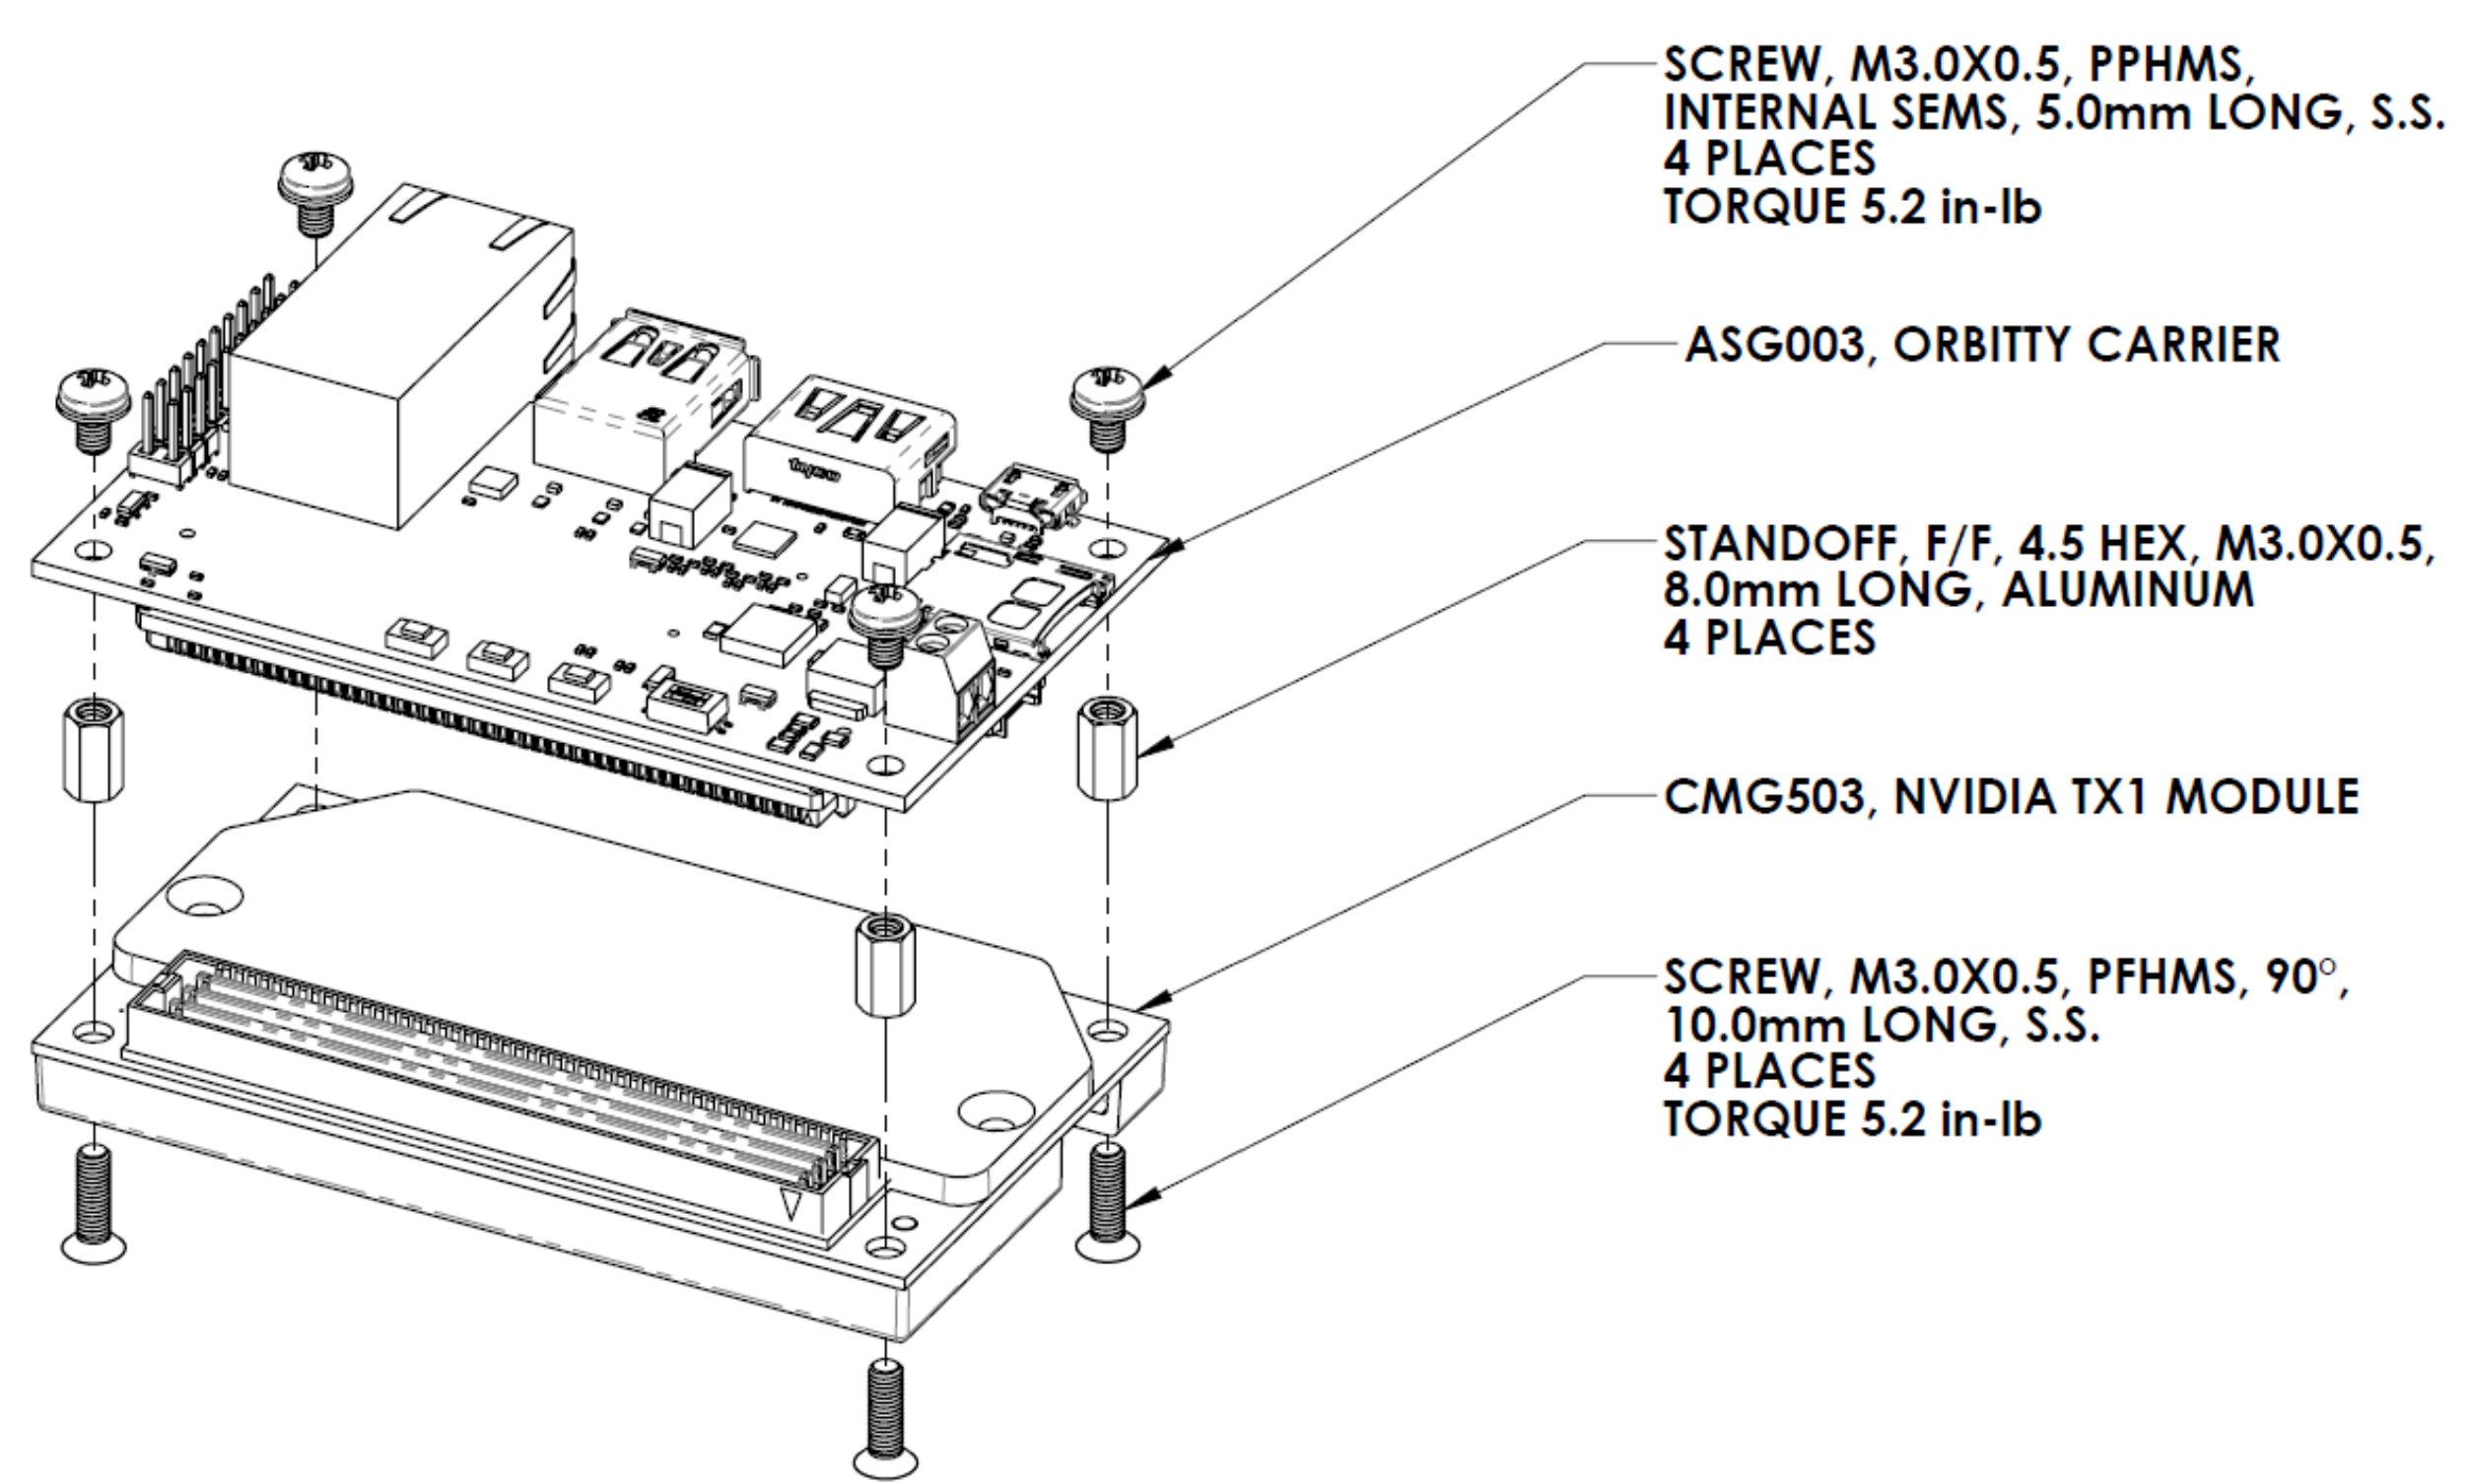
\includegraphics[width=0.75\textwidth]{Sections/LiteratureReview/img/electronics/std_jetson.png}
    \caption{Mounting diagram for NVIDIA Jetson TX2 to auxiliary board (similar mounting method is used in all other discussed electronics) \cite{dietrich_orbitty_2019}}
    \label{fig:nvidia_jetson}
\end{figure}

A comparative table of all 3 computer options is shown in Table \ref{table:computers}.

\begin{table}
    \centering
    \caption{Comparison of compute units}
    \begin{tabular}{| l | c | c | c |} \hline
        Name & Weight (g) & Power (W) & Performance
        \\ \hline
        Arduino Uno R3 & 25 & 0.232 & Low
        \\ \hline
        Raspberry Pi 4 & 46 & 5 & Medium
        \\ \hline
        Jetson TX2 & 88 & 7.5 & High
        \\
        \hline
    \end{tabular}
    \label{table:computers}
\end{table}

\sssubsection{Motor Controllers}\mbox{}\\

Motor controllers are often closed-source and are purchased specifically to be used with a certain motor.
There are also open source drivers that are designed to be compatible with a wide range of motors.

ODrive is a commonly used open-source motor driver \cite{weigl_odrive_nodate}.
Figure \ref{fig:doggo_odrive} illustrates the four oDrives used on the Stanford Doggo to actuate the 8 onboard DC motors \cite{kau_nate711/stanforddoggoproject_2019}.
Each unit can run at 24-48 V, provide over 100 A peak power per motor, and is designed to power 2 motors, giving a total power draw maximum of 480 W per motor, or 960 W per drive unit \cite{weigl_odrive_nodate}.
The drives are 135 X 50 mm and cost \$159.

\begin{figure}[H]
    \centering
    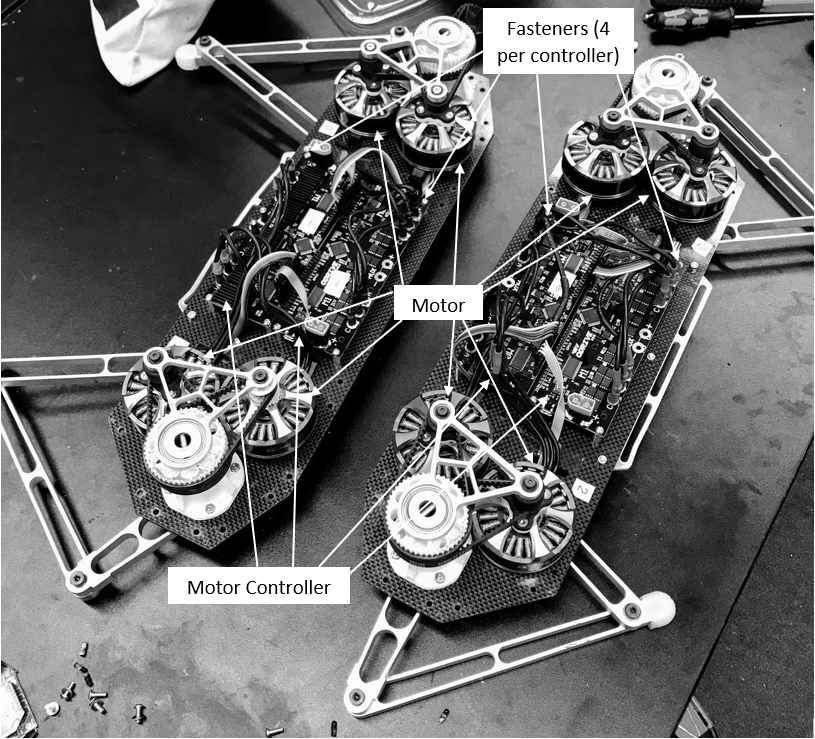
\includegraphics[width=0.9\textwidth]{Sections/LiteratureReview/img/doggo/doggo_motor_controllers.jpeg}
    \caption{Layout of oDrive motor controller of the Stanford Doggo
    \cite{kau_nate711/stanforddoggoproject_2019}}
    \label{fig:doggo_odrive}
\end{figure}

\sssubsection{Battery Pack}\mbox{}\\

While the robot may have a solar panel to provide power, the sun is not always out, meaning an auxiliary power source is necessary to run while cloudy or during the night, likely in the form of a battery power pack.
Tesla batteries are composed of 18650 cells; the 85 kWh pack contains 16 modules of 444 cells for a total of 7104 cells \cite{lambert_tear_2016}.
These have a nominal voltage of 3.7 V and capacities and discharge rates varying between 2000-3500 mAh and 5-40 A respectively \cite{18650batterystore_18650_nodate}.
The Panasonic NCR18650B cells used by Tesla cost \$4.99, have a 3400 mAh capacity and 4.9 A discharge rate.
All 18650 cells are 18.63 X 65.08 mm and weigh approximately 47.5 g \cite{18650batterystore_18650_nodate}.
They can be combined together to create higher voltage, current or capacity batteries \cite{fcbrand_building_2017}.
In this case, they require a Battery Management System to avoid overcharging and balance cell charging and discharging when in a battery \cite{engineering.com_battery_nodate} \cite{spinningmagnets_home-built_2015}.
Figure \ref{fig:18650_pack} shows a purchasable 18650 battery pack from Cult3D.

\begin{figure}[H]
    \centering
    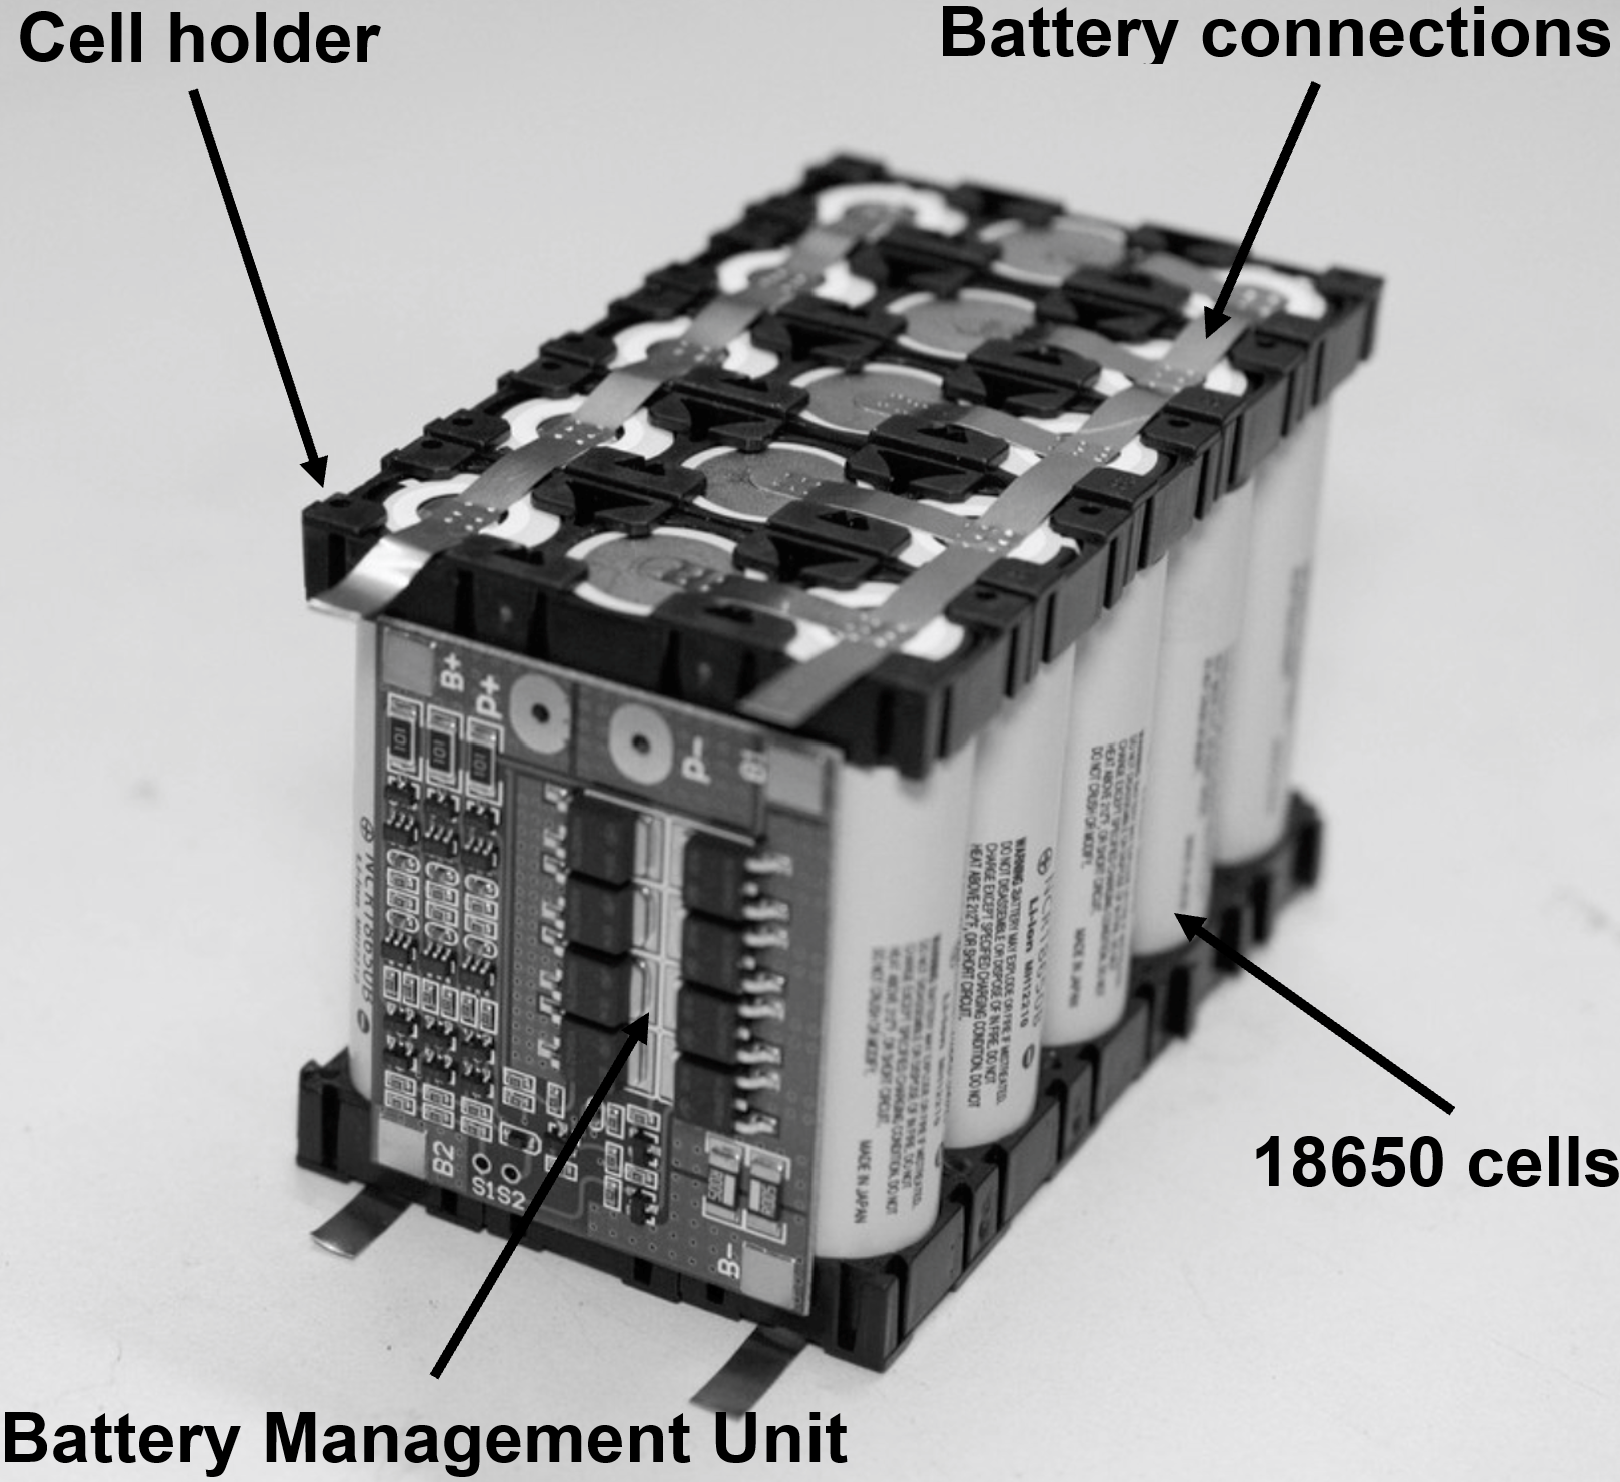
\includegraphics[width=0.6\textwidth]{Sections/LiteratureReview/img/electronics/std_18650_pack.png}
    \caption{18650 battery pack \cite{cults3d_17_nodate}}
    \label{fig:18650_pack}
\end{figure}

Battery Management systems can be purchased of the shelf for arrays of 18650 cells; OrionBMS for example offers BMS' for 24 to 168 cells in 12 cell increments, can input 8 to 30 V, consumes less than 2W and cost between \$820 and \$1680 \cite{orion_bms_orion_nodate}.
Their 24-72 cell version measures 164.9 X 158.8 X 72.6 mm and weighs 1134g.
It is mounted using 6 M2.5 screws in THRU holes.

\sssubsection{Electronics Table}\mbox{}\\

Table \ref{table:electronics} outlines the specifications of the required electronic components, for some selected options.

\begin{table} [hb!]
    \centering
    \caption{Electronics List}
    \begin{tabular}{| l | l | c | p{2.5cm} | c | p{2.5cm} |} \hline
        Role & Name & Cost (\$) & Power \newline Consumption \newline (W) & Weight (g) & Dimensions \newline (mm)
        \\ \hline
        Computer & Arduino Uno \cite{arduino_arduino_nodate} & 22 & 0.232 & 25 & 69x53x?
        \\ \hline
        Computer & Raspberry Pi 4 \cite{raspberry_pi_raspberry_nodate} & 55 & 5 & 46 & 88x58x20
        \\ \hline
        Computer & Jetson TX2 \cite{nvidia_jetson_2017} & 479 & 7.5 & 88 & 87x59x10
        \\ \hline
        GPS & Garmin GPS 15x \cite{garmin_gps_2011} & 44 & 0.263 & 7.4 & 24x43x8
        \\ \hline
        GPS/IMU & Inertial Sense $\mu$IMU \cite{inertial_sense_imu_nodate} & 800 & 0.63 & 1.3 & 17x13x5
        \\ \hline
        IMU & MPU-9250 \cite{sparkfun_sparkfun_nodate} & 15 &  N/A & N/A & 3x3x1
        \\ \hline
        Ultrasonic & MaxBotix MB7052 \cite{maxbotix_mb7052_nodate} & 203 & N/A & 15 & 35x30x25
        \\ \hline
        LiDAR & Garmin LiDAR-Lite v3HP \cite{garmin_lidar-lite_nodate} & 150 & 0.425 & 22 & 48x40x20
        \\ \hline
        Driver & oDrive \cite{weigl_odrive_nodate} & 159 & N/A & N/A & 135x50x?
        \\ \hline
        BMS & OrionBMS 24 cell \cite{orion_bms_orion_nodate} & \$820 & 2 & 1134 & 165x159x73
        \\ \hline
    \end{tabular}
    \label{table:electronics}
\end{table}

\sssubsection{Encoders}\mbox{}\\

Encoders are sensors that measure the shaft angle of rotation. These signals are used to precisely control the positioning of servo motors by analysing feedback signals and adjusting the servo motor rotation accordingly. \cite{omron_overview_nodate}

Rotary encoders such as the 1024 P/R (quadrature) produced by Karlsson Robotics, as shown in Figure \ref{fig:Encoder}, are coupled at the shaft extremity. A shaft coupling as shown in Figure \ref{fig:Coupling} is required to mount the encoder in the Figure \ref{fig:Encoder}. Note the encoder must also be mounted on a bracket not rotating with the connected shaft.

\begin{figure}[H]
    \centering
    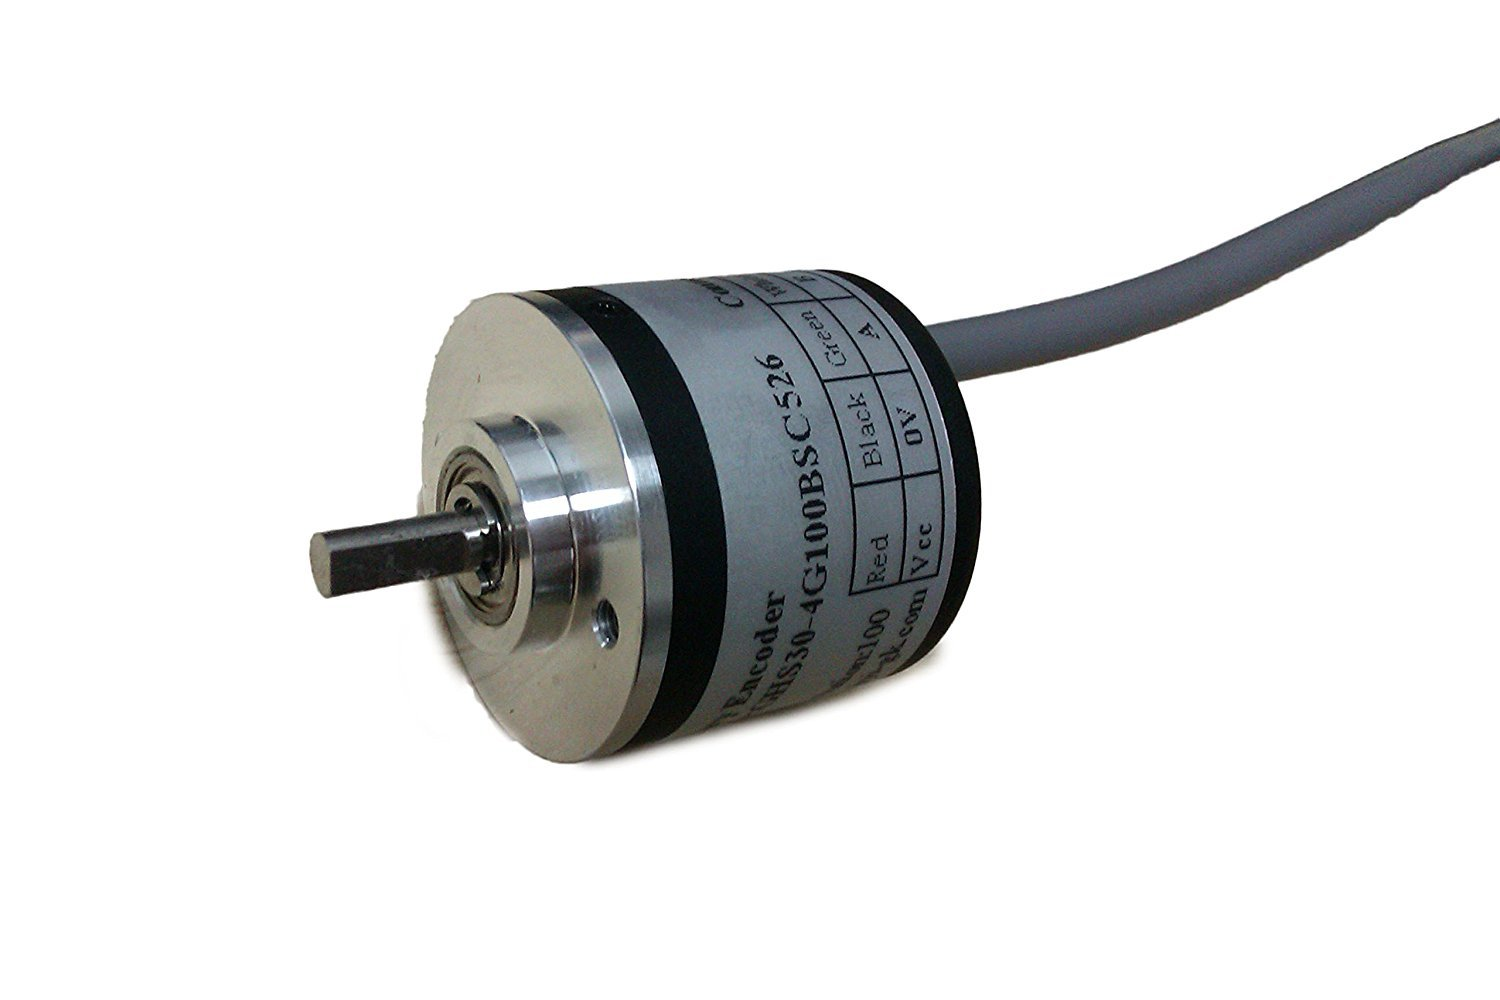
\includegraphics[width=0.6\textwidth]{Sections/LiteratureReview/img/electronics/Encoder.jpg}
    \caption{Encoder sensor with shaft \cite{amazon_rotary_nodate}}
    \label{fig:Encoder}
\end{figure}

\begin{figure}[H]
    \centering
    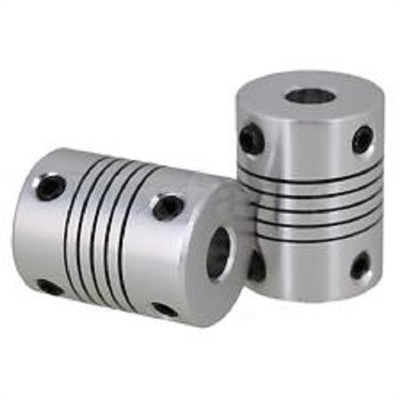
\includegraphics[width=0.4\textwidth]{Sections/LiteratureReview/img/electronics/Shaft_Coupler.jpg}
    \caption{Flexible Coupling \cite{bearings_canada_flexible_nodate}}
    \label{fig:Coupling}
\end{figure}

\sssubsection{Cable Feed Through}\mbox{}

Any electrical wire connecting to exterior components, such as  motors on leg joints, must be hermetically sealed and waterproof. Special seals, such as cable feed through must be used to seal the wires entry points as shown in Figure \ref{fig:cable_feedthrough}. 

\begin{figure}[H]
    \centering
    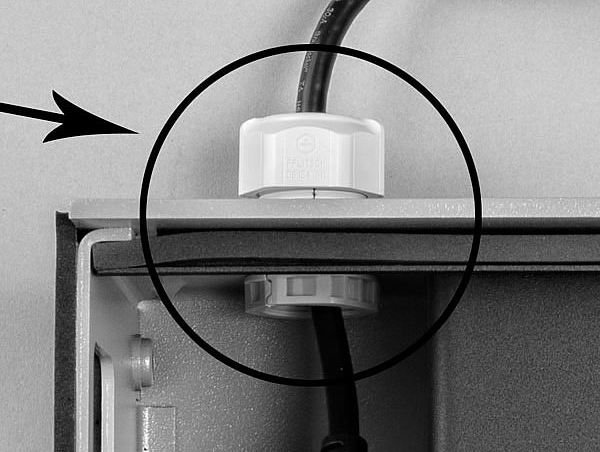
\includegraphics[width=0.4\textwidth]{Sections/LiteratureReview/cables/cable_crossSection.jpg}
    \caption{Cable feed through example \cite{garrett_1605300_nodate}}
    \label{fig:cable_feedthrough}
\end{figure}

Feed through seals can pass one or multiple wire; the connection can be parallel or perpendicular as shown in Figure \ref{fig:cable_feedthrough1} , Figure \ref{fig:cable_feedthrough2} and Figure \ref{fig:cable_feedthrough3}.

\begin{figure}[H]
    \centering
    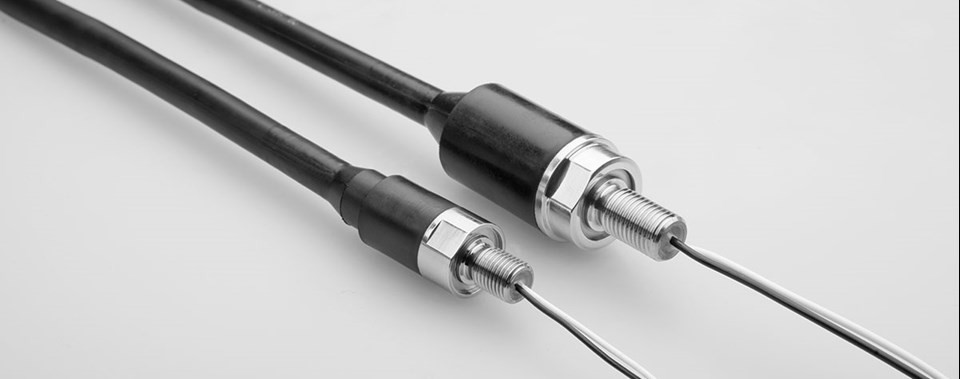
\includegraphics[width=0.4\textwidth]{Sections/LiteratureReview/cables/par_one_feed.jpg}
    \caption{Parallel one wire feed through \cite{macartney_subconn_nodate}}
    \label{fig:cable_feedthrough1}
\end{figure}

\begin{figure}[H]
    \centering
    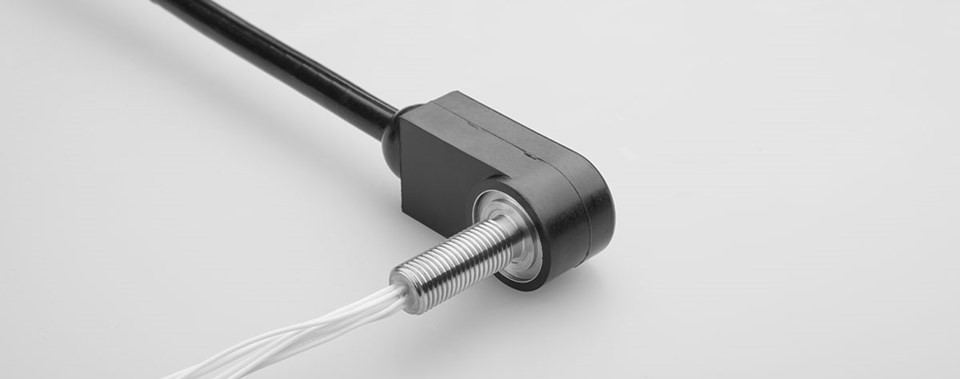
\includegraphics[width=0.4\textwidth]{Sections/LiteratureReview/cables/per_multi_feed.jpg}
    \caption{Perpendicular multiple wire feed through \cite{macartney_subconn_nodate}}
    \label{fig:cable_feedthrough2}
\end{figure}

\begin{figure}[H]
    \centering
    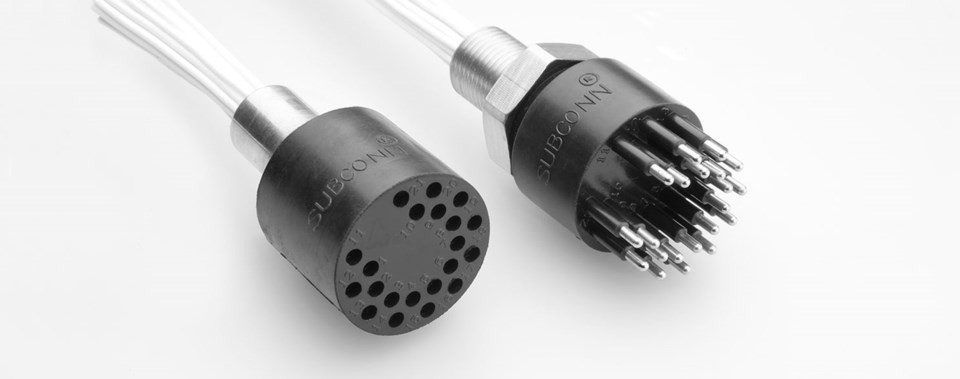
\includegraphics[width=0.4\textwidth]{Sections/LiteratureReview/cables/par_multi_feed.jpg}
    \caption{Parallel multiple wire feed through \cite{macartney_micro_nodate}}
    \label{fig:cable_feedthrough3}
\end{figure}

\newpage

